\subsection{Database Design}
\label{ssec:DB Design}
Ud fra den tekniske analyse \parencite[][Section 8]{TekniskBilag} har vi besluttet at benytte SQL til databasen. 
Projektets database har gruppen valgt at hoste i lokal storage. Dette er valgt da der under semesterets forløbet opstod problemer med skolens licens af Microsoft produkter. For at undgå at komme ud for udfordringer med hosting senere i forløbet, blev der valgt at gå med den sikre løsning, at hoste databasen lokalt på enheden. Til dette benyttede gruppen et docker image\cite{SQL server with docker}, specifikt det samme image som blev benyttet i DAB undervisning, til vores SQL server.
Hvis ikke der var problemer microsoft, havde gruppen i stedet valgt at lagre data på en cloud-based storage fremfor lokal storage.\\

\noindent For at kunne udarbejde et ER diagram til modellering af vores sql database skal vi starte med at finde ud af hvilke krav vi har til og hvilke attributter vi ønsker at gemme i vores database.\\
Først og fremmest ønskede gruppen at vi kunne gemme beskrivelserne af de forskellige rum, i spillets layout, for at formindske antallet af filer i klienten.\\ 
Her benyttes rummets id som key, da vi ikke ønsker at man skal kunne oprette flere beskrivelser til samme rum. Diagrammet kan ses på \autoref{fig:ER-Roomdescription}.

\begin{figure}[H]
\centering
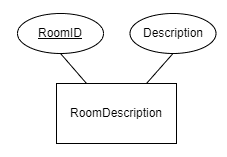
\includegraphics[width = 0.4\textwidth]{02-Body/Images/ER-RoomDescription.PNG}
\caption{ER diagram for Roomdescription. En beskrivelse består blot af en beskrivende string samt det tilhørende unikke rumid.}
\label{fig:ER-Roomdescription}
\end{figure}

\noindent Her efter kommer kravene til at kunne gemme et spil for en bruger. Her ønskede vi at man kunne stå et vilkårligt sted i spillet, med untagelse af en combat, og gemme spillet. Det skulle derefter være muligt for spilleren at loade spillet igen, hvorefter spillet er i samme stadie som man gemte det i.
ER diagrammet for at gemme et spil til en bruger på \autoref{fig:ER-GameSave}.
\begin{figure}[H]
\centering
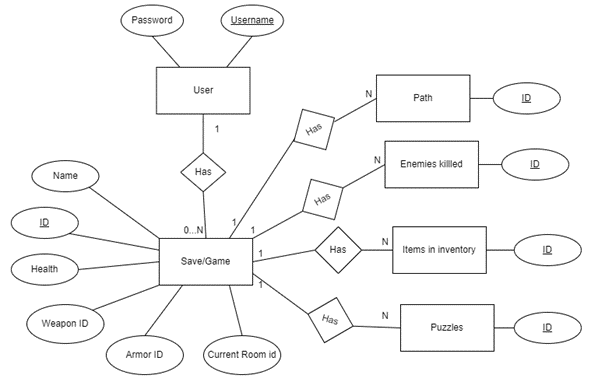
\includegraphics[width = \textwidth]{02-Body/Images/ER-GameSave.PNG}
\caption{ER Diagram til at gemme et spil til en specifik bruger. Her ses de forskellige informationer som skal til for at kunne gemme et helt spil}
\label{fig:ER-GameSave}
\end{figure}

\noindent Først og fremmest ønskede gruppen et bruger system, så eventuelle gemte spil kun tilhørte en bruger.
Der gemmes derfor en bruger entitet med et unikt brugernavn og et tilhørende password.
En spiller skal derefter kunne gemme 5 unikke spil med forskellige oplysninger, derfor overskrives der når der gemmer.\\
I et gemt spil ønkede vi at gemme en række forskellige attributter for spilleren.
Første og fremmest får hvert spil et unikt id som vi benytter til identifikation.
Et gemt spil får et navn, valgt af brugeren, som gør det nemmere for brugeren at differentiere mellem de forskellige spil. \\ 
En spillers Health og samt hvilket rum, spilleren står i gemmes.
En spiller kan derudover også holde items, såsom armor og våben, i hånden eller i sit inventory. Dette gemmes også henholdsvist som en del af et save og i en inventory liste tilhørende spillet. 

\noindent Tabellerne til højre har 2 atributter, et ID, som svarer til en bestemt item, enemy, puzzle eller rum, og en reference til et tilhørende SaveID. 
Denne parring er unik, da man ikke kan holde 2 af den samme genstand, dræbe den samme enemy, løse den samme puzzle eller gemme det samme rum til path 2 gange.\\
